\documentclass[black,white,aspectratio=169]{beamer}
\usepackage{beamerthemesplit}
\usepackage{amsmath}
\usepackage{adjustbox}
\usepackage{bookmark}
\usepackage{courier}
\usepackage[T1]{fontenc}
\usepackage{hyperref}
\usepackage[utf8]{inputenc}
\usepackage{listings}
\usepackage{lmodern}
\usepackage{tikz}
\usepackage{hyperref}
\usepackage{listings}
\usepackage{lmodern}
\usepackage{pifont}
\usepackage{subcaption}
\usepackage{svg} % Requires inkscape
\usepackage{tabularx}
\usepackage{tikz}
\usetikzlibrary{mindmap}
\usepackage{verbatim}
\usepackage{xcolor}
\usepackage{yaml}

\beamertemplatenavigationsymbolsempty
\usecolortheme{dove}
\useoutertheme{infolines}
\useinnertheme{rectangles}

\setbeamersize{text margin left=32pt,text margin right=32pt}

\newcommand{\cmark}{\ding{51}}%
\newcommand{\bigcmark}{{\large\textcolor{green}\cmark}}
\newcommand{\xmark}{\ding{55}}
\newcommand{\bigxmark}{{\large\textcolor{red}\xmark}}
\newcommand\blfootnote[1]{%
  \begingroup
  \renewcommand\thefootnote{}\footnote{#1}%
  \addtocounter{footnote}{-1}%
  \endgroup
}

\definecolor{ashgrey}{rgb}{0.7,0.75,0.71}
\definecolor{charcoal}{rgb}{0.21,0.27,0.31}
\definecolor{powderblue}{rgb}{0.69,0.88,0.9}
\definecolor{layerblue}{RGB}{213,234,254}
\definecolor{lpcyellow}{RGB}{246,243,234}
\newcommand\sectioncolor{\setbeamercolor{background canvas}{bg=lpcyellow}}

\setbeamertemplate{background canvas}[default]
\setbeamercolor{background canvas}{bg=lpcyellow}

% Align hash to font
\let\oldhash\#%
\DeclareRobustCommand{\#}{\adjustbox{valign=B,totalheight=.57\baselineskip}{\oldhash}}%

\newcommand{\link}[1]{{\large\color{blue}\href{#1}{#1}}}

% Support backup slides with their own numbering scheme
\newcommand{\backupbegin}{
   \newcounter{finalframe}
   \setcounter{finalframe}{\value{framenumber}}
}
\newcommand{\backupend}{
   \setcounter{framenumber}{\value{finalframe}}
}

\title[Packet mark in a Cloud Native world]{Packet mark in a Cloud Native world}
\institute{Cilium.io}
\author[Joe Stringer]{Joe Stringer}

\setbeamertemplate{headline}
{
    \leavevmode%
    \hbox{%
        \begin{beamercolorbox}[wd=\paperwidth,ht=2.25ex,dp=1ex,center]{}
            \insertsection
        \end{beamercolorbox}
    }
    \vskip0pt
}
\setbeamertemplate{footline}
{
    \leavevmode%
    \hbox{%
        \begin{beamercolorbox}[wd=.333333\paperwidth,ht=2.25ex,dp=1ex,left]{}%
            \usebeamerfont{date in head/foot}\hspace*{2ex}\insertshortdate{}
        \end{beamercolorbox}%
        \begin{beamercolorbox}[wd=.333333\paperwidth,ht=2.25ex,dp=1ex,center]{}%
            \usebeamerfont{title in head/foot}\insertshorttitle
        \end{beamercolorbox}%
        \begin{beamercolorbox}[wd=.333333\paperwidth,ht=2.25ex,dp=1ex,right]{}%
            \insertframenumber{} / \inserttotalframenumber\hspace*{2ex}
        \end{beamercolorbox}}%
        \vskip0pt%
}

\newcommand\newsectionpage[1]{
    \section{#1}
    {\sectioncolor
        \begin{frame}[plain]
            \vfill
            \centering
            \begin{beamercolorbox}[sep=8pt,center,shadow=true,rounded=true]{title}
                \usebeamerfont{title}\insertsectionhead\par%
            \end{beamercolorbox}
            \vfill
        \end{frame}
    }
}

\newcommand\suspense{
    \pause $\rightarrow$
}

\newcommand\todo[1]{
    \textcolor{red}{#1}
}

\newcommand{\quotebox}[1]{\begin{center}\fcolorbox{white}{blue!15!gray!15}{\begin{minipage}{0.9\linewidth}\vspace{10pt}\center\begin{minipage}{0.8\linewidth}{\space\Huge``}{#1}{\hspace{1.5em}\break\null\Huge\hfill''}\end{minipage}\smallbreak\end{minipage}}\end{center}}

\date[August 24, 2020]{}

\begin{document}
    \section*{Introduction}
    {
        \usebackgroundtemplate%
        {%
          
\includegraphics[width=\paperwidth,height=\paperheight]{background.jpg}%
        }
        \begin{frame}[plain]
            \vspace*{8ex}
            \titlepage
        \end{frame}

        % Brief self-intro
        %
        % We must have a bunch of network engineers listening in the room.
        % People who know how the internet is held together. Personally, I've
        % not been around that long so I had to google search it.
    }

    {
        \usebackgroundtemplate%
        {%
          
\includegraphics[width=\paperwidth,height=\paperheight]{internet.png}%
        }
        % https://foogle.surge.sh/
        %
        % Our amazing organizers have been encouraging us to make the most of
        % the available tooling, so I've opened up a poll for you to vote
        % which of these best represent reality. Then I guess it's really up
        % to me in this presentation to convince you all which answer I would
        % pick ;) I'll leave it open throughout the talk and we can check
        % back at the end to get a definitive answer.
        \begin{frame}
        \end{frame}
    }

    \begin{frame}{Overview}
        \tableofcontents
    \end{frame}

    \section{Background}

    \begin{frame}[fragile]{Mark of the 
\includegraphics[height=1em]{penguin.png}}
        % Let's talk about the mark of the {beast}.
        %
        % First just want to highlight that I may use any of the following
        % interchangeably. There are some subtleties to the usage for instance
        % in that the ct_mark is associated with conntrack entries rather than
        % the skb, but it's still related to this area & used commonly in some
        % of the use cases I'll present shortly.
        %
        % Despite the lack of direct commentary and otherwise innocuous-looking
        % declaration, the semantics on these bits and how they're interpreted
        % by various subsystems is really quite interesting.
        %
        % These various names hint as to the various subsystems that may be
        % involved.
        %
        % firewall mark - interestingly not just firewall (ie drop), but also
        %                 used in policy routing
        % ct mark - storable & restorable from connection tracking entries
        % socket mark - allow user applications to communicate something to
        %               kernel networking subsystems
        % xfrm mark - policy-based packet transform, eg key selection
        % pkt mark - exposed through OVS up through OVN in logical router
        %            policy.
        %
        % Also found SECMARK on my way here, but that seems to be an
        % integration specifically with SELinux security contexts and AFAICT
        % is not actually working with the mark.
        \begin{table}
            \begin{subtable}[l]{0.2\textwidth}
                \begin{itemize}
                    \item \verb+fw_mark+\medskip
                    \item \verb+skb_mark+\medskip
                    \item \verb+ct_mark+\medskip
                    \item \verb+SO_MARK+\medskip
                    \item \verb+xfrm_mark+\medskip
                    \item \verb+pkt_mark+
                \end{itemize}
            \end{subtable}
            \begin{subtable}[r]{0.7\textwidth}
                \begin{lstlisting}
                struct sk_buff {
                    ...
                    __u32 mark;
                    ...
                }
                \end{lstlisting}
            \end{subtable}
        \end{table}
        %\blfootnote{\tiny \textsuperscript{1}ct\_mark is associated with nf\_conn, but is used in conjunction with skb->mark}
    \end{frame}

    \begin{frame}{So what does the mark represent?}
        % So here's the beauty of the skb->mark. It's just some bits, which if
        % you're clued in enough on kernel networking, you can manipulate to
        % trigger various interesting paths and transfers state between different
        % subsystems.
        %
        % So here's the thing, apparently no-one thought to write it all down.
        % Was the magic too fancy? Or is everyone embarrassed about their mark
        % "hacks" so don't want to broadcast it? Or are people hiding trade
        % secrets in here?
        \begin{itemize}
            \item Nothing.. \bigskip
            \pause
            \item Anything! \bigskip
            \pause
            \item \textbf{MAGIC.} 
\includegraphics[height=1em]{sparkles.png}\bigskip
        \end{itemize}
    \end{frame}

    % Enter, stage left, Dave...
    %
    % Now, this is about as useful as its contributions. Call to action: PRs!
    % * Is this perfect? No. Mark semantics are deep, as we'll see shortly.
    % * Towards the end, maybe we'll check back in and evaluate what's here
    %   and how we might better document? Let's see.
    \begin{frame}{
\includegraphics[height=2em]{bird.png}}
        \centering
        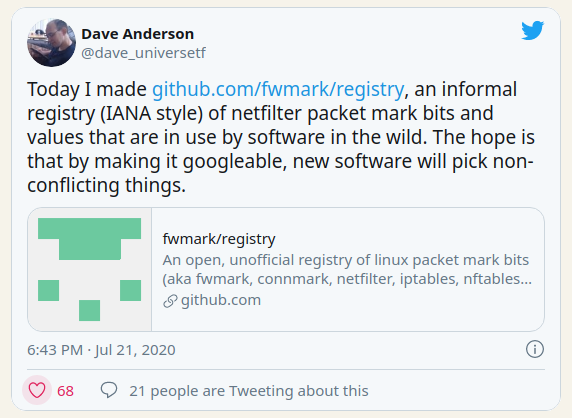
\includegraphics[height=0.5\textheight]{fwmark_tweet.png}%
        \blfootnote{{\tiny \url{https://twitter.com/dave_universetf/status/1285752332135788544}}}
    \end{frame}

    % So what's my interest? Well, I co-maintain a piece of network software
    % called Cilium which provides eBPF-based networking, security and
    % observability for cloud-native workloads.
    %
    % Cilium is a heavy user of the mark. There's a lot of features it provides
    % and many of them have ties in to the mark. I'll go into more detail on a
    % bunch of these later in the presentation. Most of the features you see
    % on the page here are somehow backed by the mark.
    %
    % Cilium is also built to be modular so that you can enable / disable
    % certain functionality. If you want to run other networking software for
    % the base networking connectivity, you're quite welcome to - we have a
    % half dozen getting started guides in the Cilium documentation for various
    % other network plugins.
    {
        \usebackgroundtemplate%
        {%
          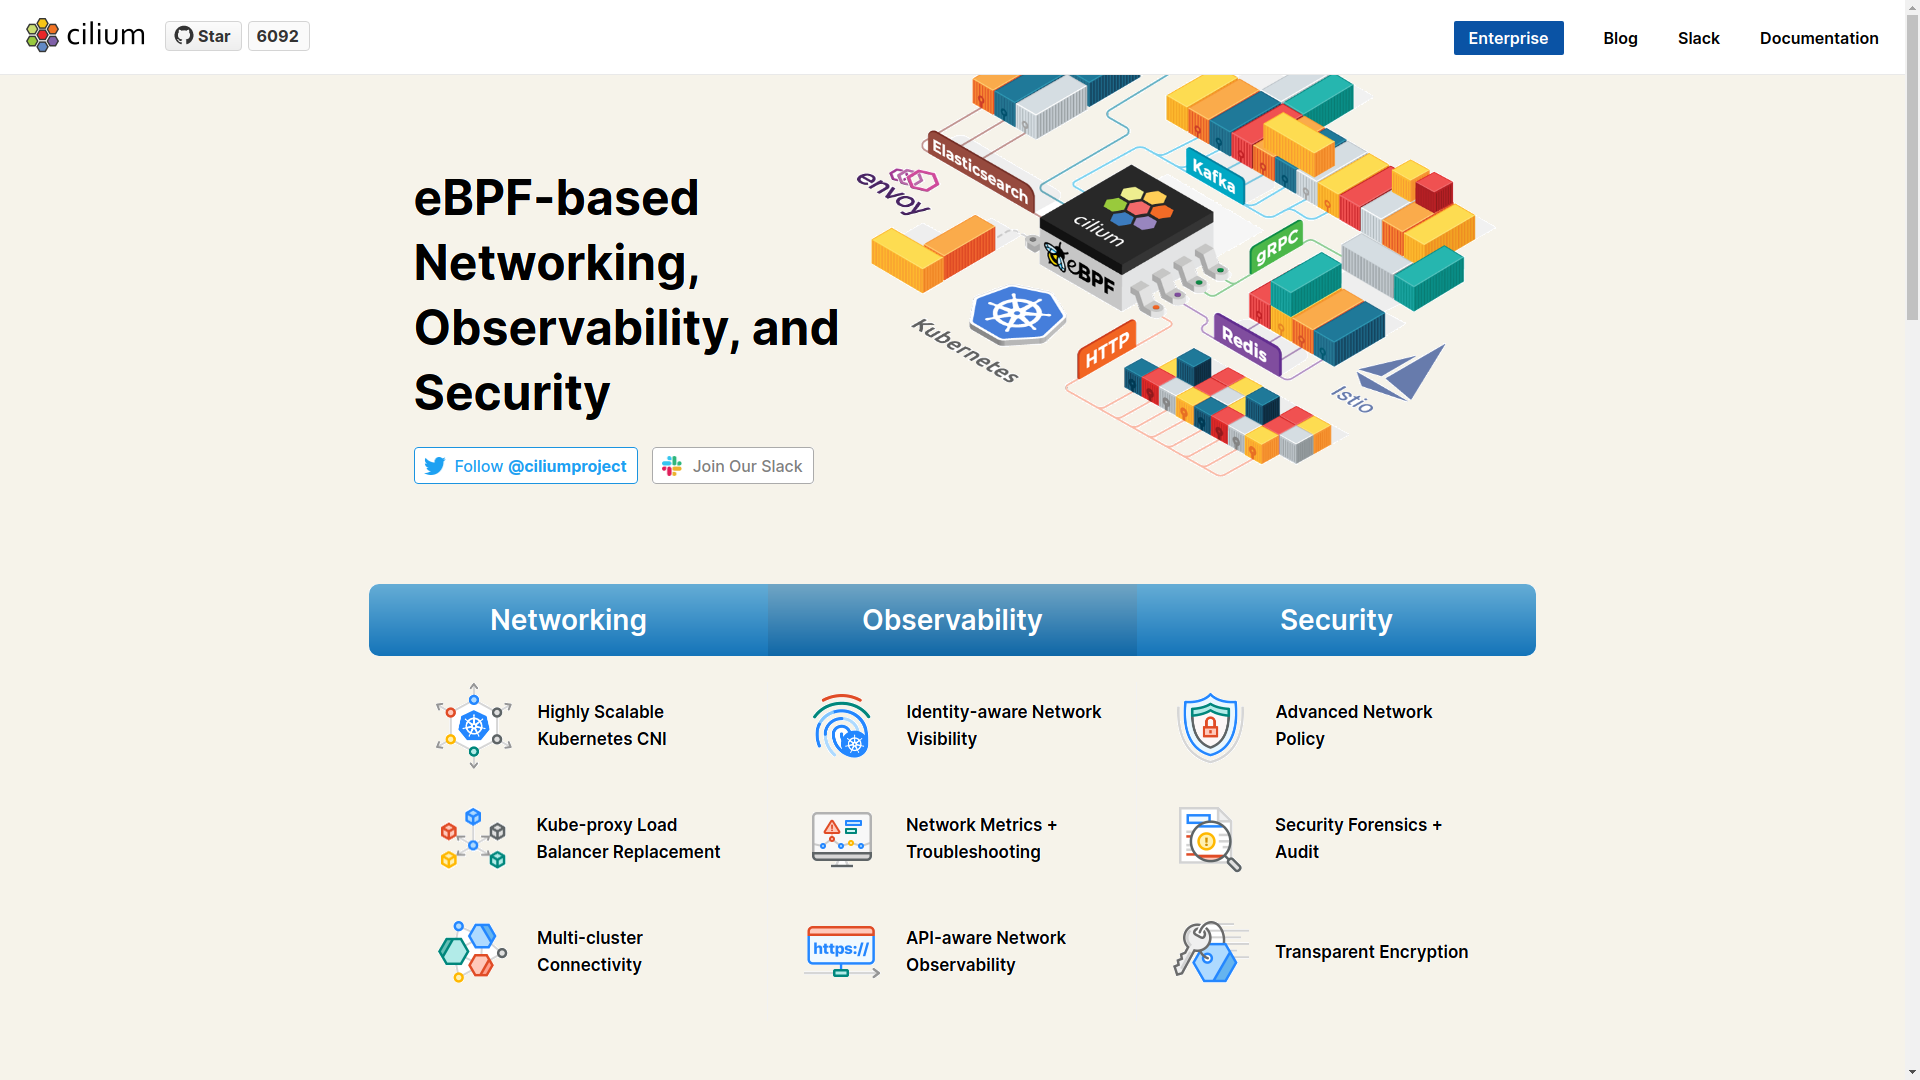
\includegraphics[width=\paperwidth,height=\paperheight]{cilium.png}%
        }
        \begin{frame}
        \end{frame}
    }

    % The thing is... there's a whole bunch of other plugins. This image is
    % for the Kubernetes space alone. It's most of the open source projects
    % out there, but it's not comprehensive. Not counting commercial projects
    % here. (But if you know how a commercial project is using the mark, it'd
    % be awesome to have that documented in the fwmark registry too!)
    %
    % *NOT* covering the whole host of other software that has been previously
    % written. There'll be some overlap and I'd welcome any discussion on that
    % at the end of the talk.
    \begin{frame}{Cloud Native networking} \begin{figure}
        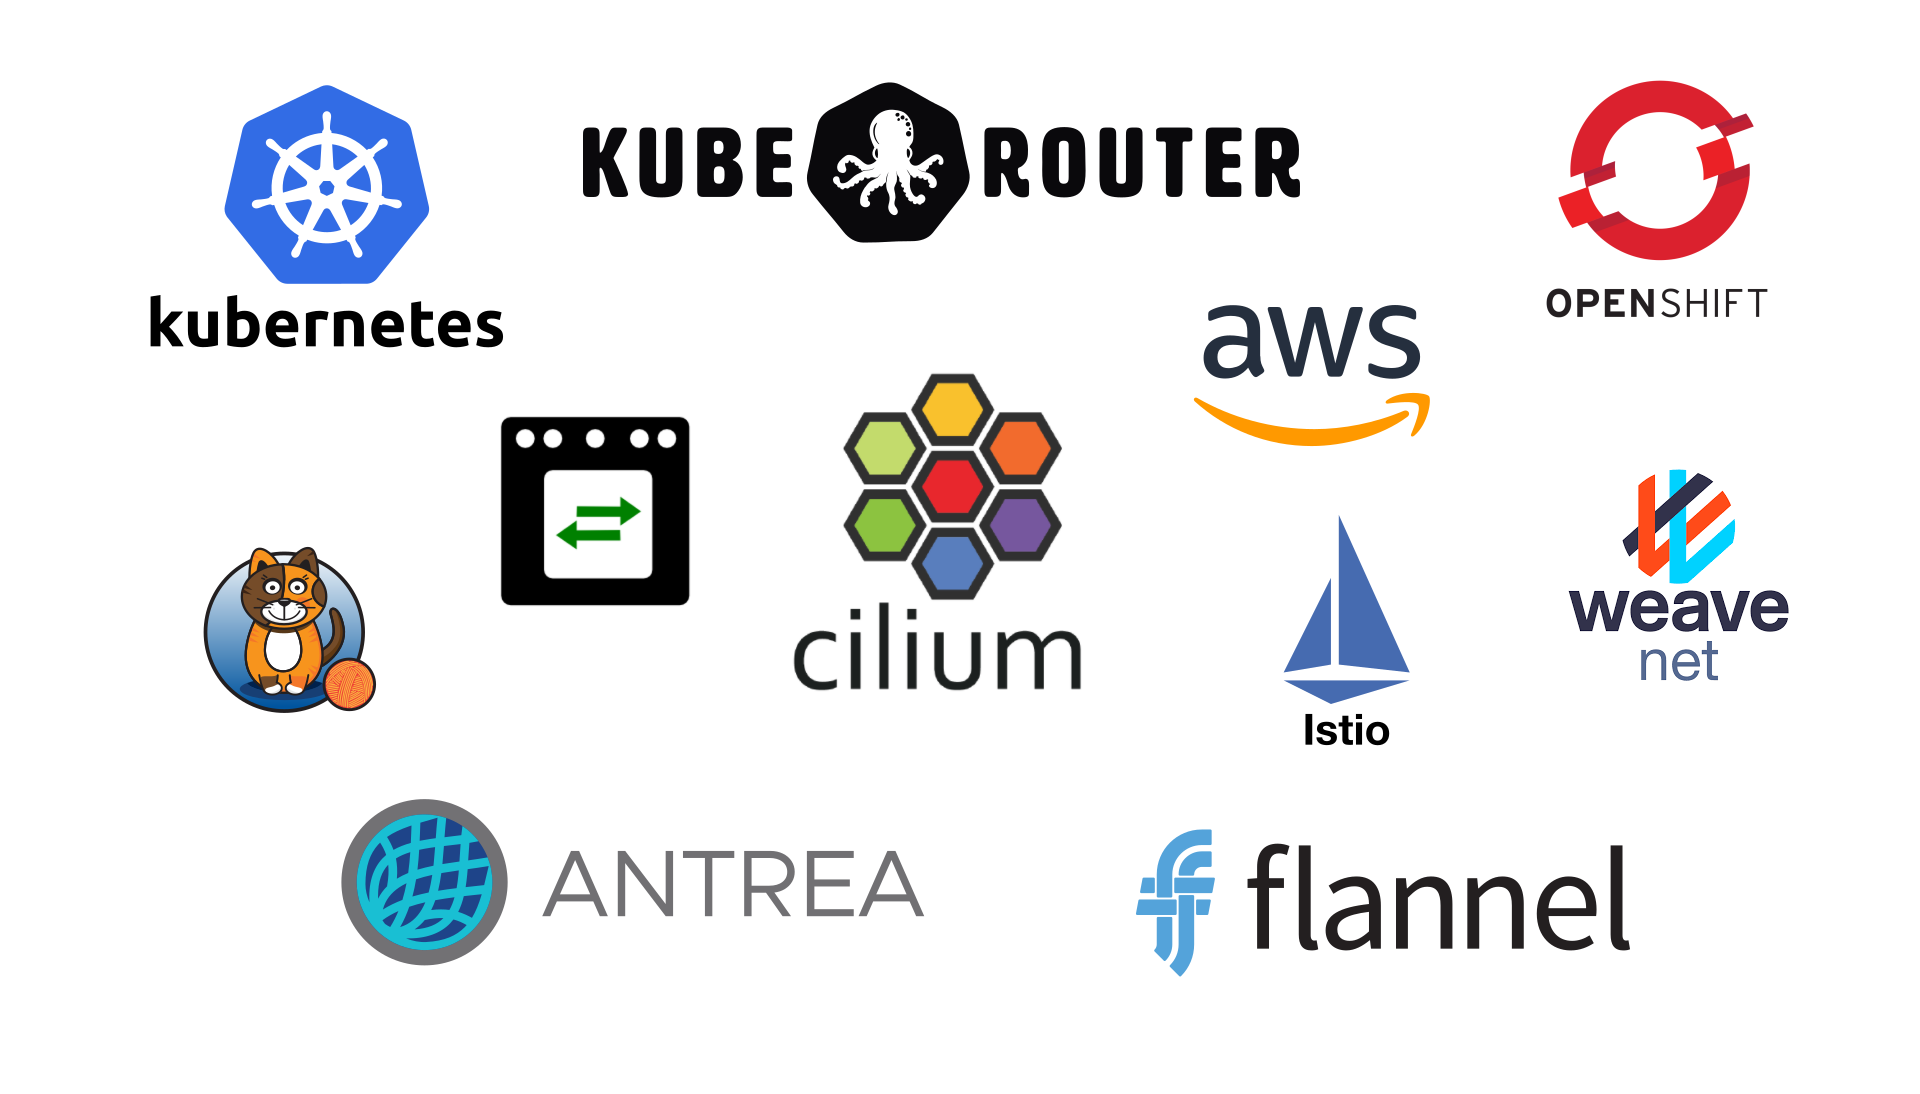
\includegraphics[width=0.85\textwidth]{plugins.png} \end{figure}
    \end{frame}

    % Rules of the game
    %
    % I mean, it's not as though this was a scientific survey..
    % Methodology or Madnessology?
    \begin{frame}{Methodology}
        \begin{enumerate}
            \item Look at CNCF landscape\footnote{\tiny \url{https://landscape.cncf.io/category=cloud-native-network&format=card-mode&grouping=category}}~\medskip
            \item Find the project on GitHub~\medskip
            \item Search for \$mark\_name~\medskip
            \item ???~\medskip
            \item Knowledge!~\medskip
        \end{enumerate}
    \end{frame}

    \newsectionpage{Use cases}

    % Let's clear out one of the most obvious cases which is built into core
    % Kubernetes itself (but also can be expanded on / replaced by CNI plugins).
    \begin{frame}{Network policy}
        \begin{itemize}
            \item 1 bit, two variations:~\smallskip
            \begin{itemize}
                \item 1 bit -> drop~\footnote{Kubernetes default}~\smallskip
                    % Honorable mention: Openstack does this, with the full
                    % 32 bits... because of course it does.
                \item 1 bit -> allow~\medskip % Weave, others
                    % Different ways to interpret this: Can be "skip policy".
            \end{itemize}
            \item Store complex path through rules into mark~\medskip
                % May be partially dependent on encryption state here, which
                % we'll get into in a bit
            \item Typically netfilter -> netfilter~\medskip
        \end{itemize}
    \end{frame}

    \begin{frame}{Transparent encryption}
        \begin{itemize}
            \item 2+ bits~\smallskip
            % {Cilium, Weave}
            \begin{itemize}
                \item 1 bit encrypt, 1 bit decrypt~\smallskip
                    % Some interesting notes here actually, in Weave case they
                    % want to only encrypt tunnel traffic between nodes in mesh.
                    % Apparently vxlan driver is not providing dst port so
                    % xfrm lookup cannot match it. Instead they do iptables
                    % match then set a mark to choose to encrypt.
                \item Variation: key selector~\medskip
            \end{itemize}
        \item \{ eBPF, netfilter \} -> xfrm~\medskip
        \end{itemize}
    \end{frame}

    \begin{frame}{Virtual IP services}
        % Antrea: Redirect traffic towards service addresses into OVS
        %         Must be for handling host traffic(?).
        % TODO: Do we need to explain {HostPort / ExternalIPs / NodePort} ?
        \begin{itemize}
            \item 1+ bits, request DNAT~\smallskip
            \begin{itemize}
                \item 1 bit: route towards bridge for DNAT~\smallskip
                \item 30 bits representing hashed 3-tuple~\medskip
            \end{itemize}
            \item \{ eBPF, netfilter \} -> routing -> netfilter~\medskip
            \item OVS -> routing -> OVS~\medskip
        \end{itemize}
    \end{frame}

    \begin{frame}{IP masquerade}
        \begin{itemize}
            \item 1+ bits, request SNAT~\smallskip
            \begin{itemize}
                \item Variation: 1 bit, Skip SNAT~\smallskip
                \item Variation: 32 bits for source address selection~\medskip
                    % OpenShift "egress traffic from this entity with external
                    % IP ___" -> full IP into mark.
            \end{itemize}
            \item Connection may not originate on the node~\medskip
            \item \{eBPF, OVS, netfilter\} -> netfilter~\medskip
                % OVS here is OpenShift + OVN.
        \end{itemize}
    \end{frame}

    % Talking about multi-homing of the nodes themselves here, not container
    % or pod multi-homing.
    %
    % Common case in cloud native tends to involve AWS just due to the way
    % they design their networking layer
    % I did see that this was used in commercial CPE type devices, including
    % openwrt. But also found one usage where this crowd-funded VPN device
    % company is shipping Javascript to shell out to iptables..
    \begin{frame}{Multi-homing}
            % I called this 'network isolation' in the talk description.
        %\item Examples: \todo{aws-vpc-cni-k8s / Cilium}
        \begin{itemize}
            \item 1 bit, two variations:~\smallskip
            \begin{itemize}
                \item Reply via primary device~\smallskip
                \begin{itemize}
                    %\item Elastic Network Interfaces (ENI) on AWS~\smallskip
                    \item Default: Pod communicates via secondary device~\smallskip
                    \item Inbound connections must reply via primary device~\smallskip
                    \item Store \& restore in connmark~\medskip
                \end{itemize}
                \item Route via management interface~\medskip
            \end{itemize}
            \item \{ socket, netfilter \} -> routing~\medskip
        \end{itemize}
    \end{frame}

    \begin{frame}{Application identity}
        % This one is fairly Cilium-specific, since we tie security policy into
        % Identity associated with the source application. But when we try
        % to integrate with other plugins that do things like either policy
        % routing (including to handle multi-homing routing for non-primary
        % devices), or even some dedicated virtual IP translation (when Cilium
        % itself is not providing that implementation), then we need some way
        % to retain that original source.
        %
        % At the destination, this Identity will be used for applying network
        % policy for traffic. Note that we may be talking about a multitenant
        % environment here where the destination has a different set of
        % policies from the source (so source is permissive while dst is not).
        %
        % This is possibly an optimization where the destination could look
        % at the source of the traffic to determine an identity. Could incur
        % a performance penalty there. Also this is stack integration cases so
        % if there are any other weird & wonderful use cases in between which
        % obscure the source IP, that approach would not be viable.
        \begin{itemize}
            \item Variable bits~\smallskip
            \begin{itemize}
                \item 4 bit pattern: ``local'' traffic~\smallskip
                \item 16+ bits: Carry Identity to destination~\smallskip
                \begin{itemize}
                    \item Policy routing~\smallskip
                    \item Portmap plugin~\medskip
                \end{itemize}
            \end{itemize}
            \item \{ eBPF, netfilter \} -> routing -> eBPF~\medskip
        \end{itemize}
    \end{frame}

    \begin{frame}[fragile]{Service proxy}
        \begin{itemize}
            \item 1+ bits depending on context~\smallskip
            \begin{itemize} % Cilium, Istio, AWS-appmesh
                \item 1 bit, route locally~\smallskip
                    % Some offenders requisitioning all 32 bits for this..
                    % Mitigation, Istio: sidecar model
                \item 16 bit tproxy port towards proxy~\smallskip
                \item 16+ bit Identity from proxy~\medskip
            \end{itemize}
            \item eBPF -> \{ netfilter, routing \}
            \item netfilter -> routing
            \item socket -> \{ eBPF, netfilter \},
        \end{itemize}
    \end{frame}

    % Consider "honorary mentions" slide
    %\begin{frame}{Honorary mentions}
    %    % Mention because they may have some place in the cloud native world,
    %    % Can't find any clear indication of existing usage in common projects.
    %    % Might be interesting to consider for implications on integration.
    %    \begin{itemize}
    %        \item Tag traffic for metrics~\medskip
    %            % IPVS + Prometheus
    %        \item Hardware offload~\medskip
    %            % Honestly I'm not sure this is a "use-case". It's an
    %            % optimization.
    %    \end{itemize}
    %\end{frame}

    \newsectionpage{Observations}

    \begin{frame}{Marking your territory}
        % Key point: Different approaches to using the mark. I own it all or
        % I have some illusion that I may be able to share it.
        %
        % Leads into... How many bits do we need?
        \begin{itemize}
            \item Bitwise usage~\smallskip
            \begin{itemize}
                \item Simpler interoperability~\smallskip
            \end{itemize}
            \item Full-mark~\smallskip
            \begin{itemize}
                \item More values to work with~\smallskip
                \item Most usage doesn't make use of this~\medskip
            \end{itemize}

        \end{itemize}
    \end{frame}

    % TODO: Come up with a better title
    %\begin{frame}{Sharing is caring}
    %\begin{frame}{No [subsystem] is an island}
    %    \begin{itemize}
    %        \item Each use case has an example of cross-system co-ordination~\smallskip
    %        \begin{itemize}
    %            \item Many cases get away with one or two bits~\smallskip
    %            \item Deviations: Where functionality is ~\medskip
    %        \end{itemize}
    %        \item Some cases resemble a stack variable~\medskip
    %    \end{itemize}
    %    \todo{Can be either within a subsystem or across subsystem components
    %          programmed by the same application}
    %\end{frame}

    \begin{frame}{A tiny bit of overload}
        \begin{itemize}
            \item Use every feature: 100+ bits~\smallskip
            \begin{itemize}
                \item ...but there's only 32 bits to play with?~\smallskip
            \end{itemize}
            \item Mitigation: Encode meaning in bit range~\smallskip
            \begin{itemize}
                \item Use [0x0000..0x000F] rather than bits in 0xFFFF~\medskip
                % Depending on how complicated you want to get, this may not work.
                % Example: "0xA" implies the uppermost 8 bits have some meaning.
                %          May be possible with eBPF, but not with routing layer.
            \end{itemize}
            \item Mitigation: Overload bits on different paths~\smallskip
            \begin{itemize}
                \item Ingress / Egress~\smallskip
                \item Make semantics dependent on packet fields~\medskip
            \end{itemize}
                % So great, now we have semantic overlap for bits in the system.
                % Can't imagine any way that's going to be a problem...
            % Which leads into how the mark usage isn't just about mark usage,
            % it's also about which fields you're matching and which order of
            % features / rules you hit, which combination of subsystems you
            % hit, 
        \end{itemize}
    \end{frame}

    \begin{frame}{One does not simply understand skb->mark}
        % Mark doesn't operate in a vacuum. Ultimately you must not only
        % understand whether to set/not set specific bits, but depending on
        % which features you intend to reuse, you may need to understand how
        % other logic is triggered.
        %
        % There's this other aspect here where it's really up to each project
        % that cares to figure out the potential bitwise conflict with other
        % individual projects.

        \vfill
        \begin{table}
            \begin{subtable}[l]{0.7\textwidth}
                \begin{itemize}
                    \item Required reading: network stack diagram~\medskip
                    \item Distinct bits do not guarantee integration~\smallskip
                    \begin{itemize}
                        \item skb, conn matches may steer packets~\medskip
                    \end{itemize}
                     \item Fun: replies disappear~\medskip
                     \item Proxies: Double the connections, double the fun~\medskip
                \end{itemize}
            \end{subtable}
            \begin{subtable}[r]{0.25\textwidth}
                
\includegraphics[width=0.6\textwidth]{boromir.jpg}
            \end{subtable}
        \end{table}
        \vfill
    \end{frame}

    \newsectionpage{Evaluation}

    % TODO: Revisit this:
    % I think we're trying to answer the question "Does the mark work?" here.
    % Obviously it is functional for specific use cases, but does it broadly
    % provide an interoperability story for network control software?

    \begin{frame}{Properties of skb->mark}
        \begin{itemize}
            \item Powerful mechanism for cross-subsystem programming~\medskip
                % No predefined semantics assignment. Lots of freedom to define
                % those when programming the kernel.
            \item Frequent uncertainty whether bits are OK to use~\medskip
                % Hopefully the fwmark registry will help with this, but that
                % relies on your participation, hint hint!
            \item Can be a crutch~\medskip
                % Starts out fixing this one hacky case, ends up with mark overload
            \item When you run out of bits, the ``fun'' starts~\medskip
                % Both from design perspective but also from deploy/debug cycle
        \end{itemize}
    \end{frame}

    \begin{frame}{Interoperability}
        \begin{itemize}
            \item Driven by common deployment scenarios~\medskip
                % All Kubernetes networking plugins respect bit 15: DROP
                %
                % It's difficult to arbitrarily support integration with other
                % plugins, because you don't necessarily know the ways that
                % they're configuring the stack.
            \item The clearer responsibility assignment you have, the better~\medskip
                % Example: When Cilium provides just network policy on top of
                %          another plugin for connectivity, we know we won't
                %          have to configure the encryption bits.
                %
                % More difficult is when you're integrating with arbitrary
                % iptables rules so you don't know if your traffic will be
                % messed with and you also don't know if the mark will be
                % thrashed...
            \item Not free (in effort or in complexity)~\medskip
            % What features do you need / what are you trading off?
            % \item At what point do you lose the benefit of independent
            %       software implementations and should just implement the
            %       functionality yourself?
        \end{itemize}
        %\todo{Eg most of these software must work with k8s. Default configuration
        %      makes BIT 15 -> Drop.} \bigskip
        %\todo{Scope changes depending on how ambitious you are. Cilium aims to
        %      allow swapping in/out routing / service layers.
        %      Means that when you run alternative implementation, there must be
        %      co-ordination.} \bigskip
    \end{frame}

    % Many features

    \begin{frame}{Mitigating conflicts}
        \begin{itemize}
            \item ``If only I had more bits...''~\medskip
            \item How can we get more?~\smallskip
            \begin{itemize}
                \item Extend the kernel..~\smallskip
                    % Not ruling this out, but I'm also aware there are other
                    % potential avenues to explore.
                %    \todo{CONFIG\_SKB\_EXTENSIONS}
                \item Consolidate datapath usage within primary subsystem~\medskip
                    % Ie don't split half your logic into iptables. Embrace
                    % eBPF if that's where you're at. Or embrace OVS if that's
                    % what you use.
                %\item \todo{tproxy eBPF - saved 16 bits of 32-bit mark} \bigskip
                %\item \todo{floated - eBPF/xfrm} \bigskip
            \end{itemize}
        \end{itemize}
    \end{frame}

    % There's some interesting angle here for Cilium's perspective. We've been
    % able to flesh out a whole bunch of use cases by making use of the mark,
    % occasionally maximising the number of bits such that some combinations of
    % features cannot be enabled at the same time. The great thing here is that
    % we can build out that support on any kernel version.
    %
    % Downsides: Debuggability, less ability to integrate due to mark overload,
    % related: maintenance, education. More complex. Now we're starting to look
    % at specific directions where we can extend eBPF to provide primitives
    % that allow us to simplify (``remove boxes'' from arch diagram) and
    % optimize performance by eliminating unnecessary infrastructure.
    %
    % One of the big angles we're looking at now is to move the last few bits
    % of iptables usage into eBPF directly.

    \section*{Summary}
    \begin{frame}{Summary}
        \begin{itemize}
            \item Cloud native use cases~\medskip
            \item Challenges for interoperability~\medskip
                % And how about you?
            \item Mitigations \& dangers~\medskip
        \end{itemize}
    \end{frame}

    % Now I'm curious to hear from you. What did I miss?
    \begin{frame}[plain]{}
        \centering
        \vfill
        \begin{table}
            \begin{subtable}[l]{0.6\textwidth}
                \begin{tabular}{rl}
                    \multicolumn{2}{l}{\textbf{Cilium}} \\ \\
                    \includesvg[width=0.045\textwidth]{www.svg}
                    & \link{https://cilium.io} \\
                    \includesvg[width=0.045\textwidth]{slack.svg}
                    & \link{https://cilium.io/slack} \\
                    \includesvg[width=0.045\textwidth]{github.svg}
                    & \link{https://github.com/cilium/cilium} \\
                    \includesvg[width=0.045\textwidth]{twitter.svg}
                    & \link{https://twitter.com/ciliumproject} \\ \\
                    \multicolumn{2}{l}{\textbf{Mark registry}} \\ \\
                    \includesvg[width=0.045\textwidth]{github.svg}
                    & \link{https://github.com/fwmark/registry} \\
                \end{tabular}
            \end{subtable}
            \begin{subtable}[r]{0.3\textwidth}
                \includesvg[width=\textwidth]{cilium-gopher.svg}
            \end{subtable}
        \end{table}
        \pause
        \vfill
    \end{frame}

    \appendix
    \backupbegin

    \section*{Appendix}
    \begin{frame}{Backup Slide}
    \end{frame}

    \backupend

\end{document}
